%%%%%%%%%%%%%%%%%%%%%%%%%%%%%%%%%%%%%%%%%%%%%%%%%%%%%%%%%%%%%%%%
\begin{frame}[fragile]\frametitle{}
\begin{center}
{\Large Zenoga}


{\tiny (Based on ``Zen Yoga'' by P J Saher And Deep Knowledge YouTube Channel by Dr Ashish Shukla)}
\end{center}
\end{frame}


%%%%%%%%%%%%%%%%%%%%%%%%%%%%%%%%%%%%%%%%%%%%%%%%%%%%%%%%%%%%%%%%
\begin{frame}[fragile]
\frametitle{Prelude}

\begin{columns}[T] % align columns
\begin{column}{.48\textwidth}
\begin{itemize}
\item Mind is divided into 4 sections
	\begin{itemize}
	\item Section 1 : Brain
	\item Section 2 a: RAS
	\item Section 2 b:
	\item Section 3
	\item Section 4
	\end{itemize}
\item Lower Dimension: 1, 2a
\item Higher Dimension: 2b, 3, 4
\end{itemize}
\end{column}%
\hfill%
\begin{column}{.48\textwidth}
 \begin{center}
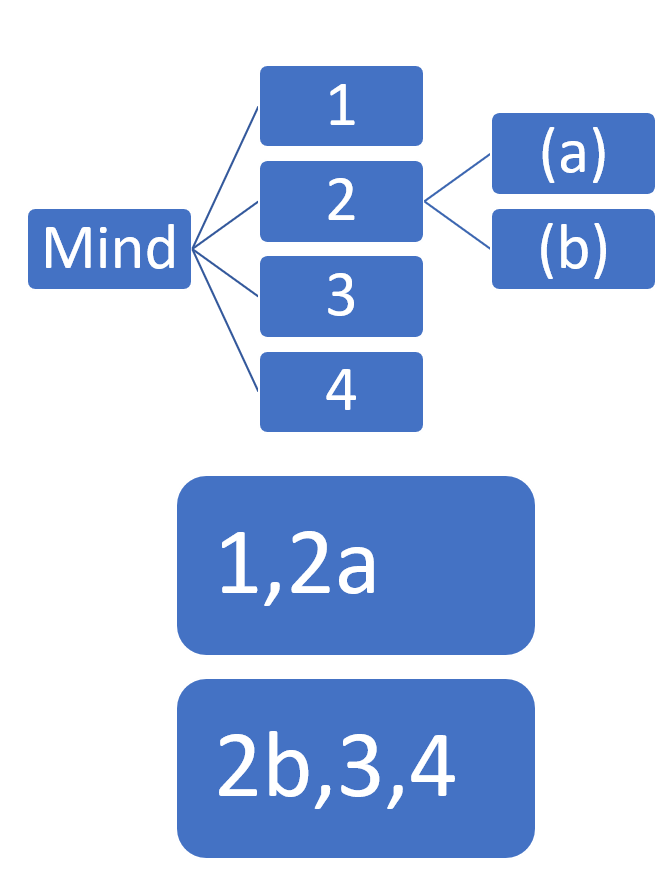
\includegraphics[width=0.9\linewidth,keepaspectratio]{images/zenyoga1}
\end{center}

\end{column}%
\end{columns}
\end{frame}

%%%%%%%%%%%%%%%%%%%%%%%%%%%%%%%%%%%%%%%%%%%%%%%%%%%%%%%%%%%%%%%%
\begin{frame}[fragile]\frametitle{}
\begin{center}
{\Large Notes from Other References}
\end{center}
\end{frame}


%%%%%%%%%%%%%%%%%%%%%%%%%%%%%%%%%%%%%%%%%%%%%%%%%%%%%%%%%%%%%%%%
\begin{frame}[fragile]
\frametitle{``Introduction To Three Step Rhythmic Breathing(3SRB)'' by Mr.Deepak Dhingra}


\begin{itemize}
\item Yaksh : ``What's the most delusion that humans have?''
\item Yudhishthiara: ``People live life as if they are not going to die''.
\item Its inevitable. No one has control. 
\item Only sometimes externally.
\item But we have no control internally. 
\end{itemize}
\end{frame}


%%%%%%%%%%%%%%%%%%%%%%%%%%%%%%%%%%%%%%%%%%%%%%%%%%%%%%%%%%%%%%%%
\begin{frame}[fragile]
\frametitle{Mind}
\begin{itemize}
\item None of the internal organs behave the way we want. 
\item Including brain!! although we believe we have control on that
\item Brain is just another organ, a hardware. And mind is the energy/software that runs on it.
\item Proof: After death, hardware remains, but the software/energy is shutdown, so cant function.
\end{itemize}
\end{frame}



%%%%%%%%%%%%%%%%%%%%%%%%%%%%%%%%%%%%%%%%%%%%%%%%%%%%%%%%%%%%%%%%
\begin{frame}[fragile]
\frametitle{Free Will?}

\begin{itemize}
\item We have no control internally. Many centers are producing impulses. Most of the organ functioning is autonomous
\item Thus we cannot control mind, but we have to bring them to rhythm, balance.
\item As per Pantanjali, daily, out of 13k impulses 120 go to brain. Rest are used to keep system working. Out of 120 to brain, 12 are per second, Only one becomes a thought. This just one more theory. May ignore. Just a model.
% \item We are interpreting life our way and not how it is
\end{itemize}
\end{frame}

%%%%%%%%%%%%%%%%%%%%%%%%%%%%%%%%%%%%%%%%%%%%%%%%%%%%%%%%%%%%%%%%
\begin{frame}[fragile]
\frametitle{Mind}
\begin{itemize}
\item As per Patanjali, Breathing is one way to control the mind.
\item Breathing happens as per emotions, eg. anger.
\item Can controlling breathing control emotions? Patanjali says, Yes.
\item Mind (Software) is run by breath. When Breath stops, its called death.
\item Need Deep, Rhythmic and Belly breathing
\end{itemize}
\end{frame}

%%%%%%%%%%%%%%%%%%%%%%%%%%%%%%%%%%%%%%%%%%%%%%%%%%%%%%%%%%%%%%%%
\begin{frame}[fragile]
\frametitle{3SRB (3 Step Rhythmic Breathing )}

Technique

\begin{itemize}
\item Both chest and abdomen are raised and lowered together equally.
\item Note: You can lie down in front of the mirror with two heavy books one on the chest and the other on the abdomen. 
\item Check whether both move together.
\end{itemize}

\tiny{(Ref: https://www.3srb.org/3srb/how-to-practise-3srb.html )}
\end{frame}

%%%%%%%%%%%%%%%%%%%%%%%%%%%%%%%%%%%%%%%%%%%%%%%%%%%%%%%%%%%%%%%%
\begin{frame}[fragile]
\frametitle{3SRB (3 Step Rhythmic Breathing )}

Volume

\begin{itemize}
\item The breath is full from neck to naval, i.e. the upper, middle and lower abdomen are filled to normal capacity
\item The quantum of air inhaled and exhaled is what is usually normal to us neither too much nor too forceful, since normal 3SRB is not an exercise but a process of correct breathing. 
\item Note: Initially, to establish the rhythm your breath will be deeper. Once, the technique and volume is mastered, then the volume of the breath will be normal as you breath today.
\end{itemize}
\end{frame}


%%%%%%%%%%%%%%%%%%%%%%%%%%%%%%%%%%%%%%%%%%%%%%%%%%%%%%%%%%%%%%%%
\begin{frame}[fragile]
\frametitle{3SRB (3 Step Rhythmic Breathing )}

Rhythm

\begin{itemize}
\item In 3 sec out 2 sec | one hand chest one hand on belly| equal volume. No jerks. 
\item  While counting its 1-2-3 (4) 5-6. Here, at ``4'' it is the turn of breath. Is not counted but just understood. Later, same but with deep breathing, and fast
\item 12 cycles a minute to start with then to 24 and 36.
\item  Increase the duration of practice by 5 minutes every fortnight until 6 months time and until one hour of conscious 3SRB is reached.
\end{itemize}
\end{frame}


%%%%%%%%%%%%%%%%%%%%%%%%%%%%%%%%%%%%%%%%%%%%%%%%%%%%%%%%%%%%%%%%
\begin{frame}[fragile]
\frametitle{3SRB by ShriRajen Vakil}


\begin{itemize}
\item Deep Chest breathing: Both hands on chest. Let breath come in and push chest out. 36 times a minute. Only for a minute. On rhythm 123-56. Area of anger, jealousy stored so far.
\item Deep Stomach breathing: Both hands on belly. Let breath come in and push belly out. On exhale push belly in. 36 times a minute. Only for a minute. On rhythm 123-56. Area of fear and worry for future.
\item Paschimottanasan breathing: Head up. Both chest and stomach should come out on breath in. 36 times a minute. Only for a minute. On rhythm 123-56. For backbone, the channel for energy to go up.
\item Take breath in 5 installments and breath in through mouth forcefully. 12345-Out
\item Breath in 5 seconds, hold 5, empty 5, hold 5. 3 such rounds.
\item Inhale, hold breath, touch chin, swallow 5 times. Area of Pain.

\end{itemize}
\end{frame}

%%%%%%%%%%%%%%%%%%%%%%%%%%%%%%%%%%%%%%%%%%%%%%%%%%%%%%%%%%%%%%%%
\begin{frame}[fragile]\frametitle{}
\begin{center}
{\Large Conclusion}
\end{center}
\end{frame}



%%%%%%%%%%%%%%%%%%%%%%%%%%%%%%%%%%%%%%%%%%%%%%%%%%%%%%%%%%%%%%%%
\begin{frame}[fragile]
\frametitle{Summary To-Dos}
\begin{itemize}
\item Breath: Three Step Rhythmic Breathing
\item Food: lessen intake slowly to 1 time, be aware, get rid off addiction
\item Drift: Watch thoughts-wavering, Put in Fear/Anger/Sex/Hope/Jealousy
\item Walking with Awareness: 
\item Corrective methods: replace negative with positive thoughts
\item Sleep: 11 pm to 5 am. Other times do 3 step breathing
\item Reading
\item Sex Moderation
\item Awareness of Eyes: watch carefully, focus
\item Awareness of Ears: listen carefully, don't drift
\end{itemize}
\end{frame}
